\documentclass[onecolumn, draftclsnofoot,10pt, compsoc]{IEEEtran}
\usepackage{graphicx}
\usepackage{url}
%\usepackage{setspace}

\usepackage{geometry}
\geometry{textheight=9.5in, textwidth=7in}


% 1. Fill in these details
\def \CapstoneTeamName{			Addax}
\def \CapstoneTeamNumber{		38}
\def \GroupMemberOne{			Caitlyn Cook}
\def \GroupMemberTwo{			Iliana Javier}
\def \GroupMemberThree{			Nicholas Skinner}
\def \GroupMemberFour{			Amy Tang}
\def \CapstoneProjectName{		Impala performance tuning on HDFS}
\def \CapstoneSponsorCompany{	Hewlett Packard}
\def \CapstoneSponsorPerson{	Andy Weiss}

% 2. Uncomment the appropriate line below so that the document type works
\def \DocType{		Project Update Winter 2019
				%Research Proposal Document
				%Technology Review
				%Design Document
				%Progress Report
				}
			
\newcommand{\NameSigPair}[1]{\par
\makebox[2.75in][r]{#1} \hfil 	\makebox[3.25in]{\makebox[2.25in]{\hrulefill} \hfill		\makebox[.75in]{\hrulefill}}
\par\vspace{-12pt} \textit{\tiny\noindent
\makebox[2.75in]{} \hfil		\makebox[3.25in]{\makebox[2.25in][r]{Signature} \hfill	\makebox[.75in][r]{Date}}}}
% 3. If the document is not to be signed, uncomment the RENEWcommand below
%\renewcommand{\NameSigPair}[1]{#1}

%%%%%%%%%%%%%%%%%%%%%%%%%%%%%%%%%%%%%%%
\begin{document}
\begin{titlepage}
    \pagenumbering{gobble}
    %\begin{singlespace}s
    	\includegraphics[height=4cm]{coe_v_spot1}
        \hfill 
        % 4. If you have a logo, use this includegraphics command to put it on the coversheet.
        %\includegraphics[height=4cm]{CompanyLogo}   
        \par\vspace{.2in}
        \centering
        \scshape{
            \huge CS Capstone \DocType \par
            {\large\today}\par
            \vspace{.5in}
            \textbf{\Huge\CapstoneProjectName}\par
            \vfill
            {\large Prepared for}\par
            \Huge \CapstoneSponsorCompany\par
            \vspace{5pt}
            {\Large\NameSigPair{\CapstoneSponsorPerson}\par}
            {\large Prepared by }\par
            Group\CapstoneTeamNumber\par
            % 5. comment out the line below this one if you do not wish to name your team
            \CapstoneTeamName\par 
            \vspace{5pt}
            {\Large
                \NameSigPair{\GroupMemberOne}\par
                \NameSigPair{\GroupMemberTwo}\par
                \NameSigPair{\GroupMemberThree}\par
                \NameSigPair{\GroupMemberFour}\par
            }
            \vspace{20pt}
        }
        \begin{abstract}
        % 6. Fill in your abstract    
            The Big Data team at Hewlett Packard currently uses an Oracle database to store industrial IoT data gathered from large printing presses. 
            They are interested in moving from their current centralized database to a distributed architecture, and have asked our team to investigate the operation of their planned system.
            This report introduces our project, defines our goals, discusses the work completed during Fall and Winter Terms, and discusses some challenges encountered during Winter term.
        \end{abstract}     
    %\end{singlespace}
\end{titlepage}
\newpage
\pagenumbering{arabic}
\tableofcontents
% 7. uncomment this (if applicable). Consider adding a page break.
%\listoffigures
%\listoftables
\clearpage

% 8. now you write!
\section{Project Description}
\subsection{Background}
The HP BackOffice database stores data collected from approximately 300 industrial printers, called web presses, in operation globally.
The presses print on paper up to 110 in wide at the largest, and are capable of printing at speeds of up to 1000 ft per minute in full color.
The presses are used to print books, packaging, and mail at an industrial scale for many major companies.
For example, the presses are a part of how Amazon is able to print and ship a brand new copy of a book within 4 hours of ordering it on their website.

Each press records data that is used to diagnose issues, study press operation, and guide the development of new features.
Data is collected on alarms, pen health, print jobs, and other aspects of operations.
This data is streamed to HP's database, where it is processed and analyzed by teams of engineers.
New data is added to the database at a rate of approximately 60 - 100 GB per day; currently, the database holds approximately 30TB of data. 

HP's current database is a centralized Oracle 12c database which shares all memory and disk resources between multiple processors.
While Oracle databases handle transactions extremely well, HP doesn't have much need for transactions. 
Their data is static once written; once the data for a day is collected and stored, it is not further modified.
Instead, HP mostly performs analytic processing on their data, which suffers unnecessarily from the overhead that makes Oracle so good at transactions.
The monolithic architecture of their current database also presents difficulties with scaling.
As HP anticipates future data loads, they want a solution that will allow cheaper and more efficient scaling.
This is their motivation behind our project; we are to investigate the behavior of a distributed system which will fare better in these key areas.
Our research will result in information that will help ease their transition process.

\subsection{Purpose}
HP's data team has tasked us with gathering information about a distributed database system implementation. 
The data team is particularly interested in Apache / Cloudera Impala, a SQL engine that runs on the popular Hadoop Distributed File System (HDFS), and would like us to focus on researching this engine's mechanisms. 

Our sponsor has a variety of reasons for being interested in distributed database systems.
At the core of every business and engineering decision is cost, in terms of both time and money.
In terms of time, HP's current exponentially growing database is causing queries to result in long running times.
This is due simply to the large amount of data tables that need to be scanned, reduced, or joined by the single server.
In addition, there is significant slowdown caused by the overhead Oracle implements for each query.
This work could be eased by implementing a system that distributes queries across multiple servers.
HP has also spent years understanding and optimizing their SQL queries to best fit their data's behavior, so they would like any new system they adopt to run SQL as well.
Apache Impala fits these criteria.
Monetarily, HP is interested in moving to an open source solution to cut the cost of Oracle's software licensing fees, which grow more expensive the more data the database houses.
Impala, as well as its underlying Hadoop system, is open source. 
These criteria make Impala a promising solution for HP's data problems.

\subsection{Goals}
The goal of our project is to produce a document that will guide a person familiar with shared-everything database architectures through the setup and use of a shared-nothing architecture.
We will focus on multiple aspects of the system and provide an explanation of their function which will allow the reader to examine and improve the performance of a distributed system.
In particular, this document will examine the tools available for diagnosing and tuning performance problems, the metadata store of the database, the generation of query plans and how parallelization across nodes affects these plans.
We will accomplish this through a combination of experimentation and reading existing documentation.

\subsection{Challenges}
Last term, we had the challenge of defining our own assignments.
This term, we have taken one of the assignments produced last term and expanded it to fulfill the requirements of our final deliverable for HP.
Modifying the existing document has produced some challenges, as our audience for the paper has shifted from Capstone graders to HP’s team.
We have also encountered some difficulty answering questions we intended to write about that were not explicitly addressed by documentation or other research.
To answer these questions, we have had to broaden the scope of our search as well as do some experimentation of our own. 

We have also been challenged this term to represent our project in accessible terms, through both a poster and elevator pitches.
Our project has proven difficult to explain in simple terms, as it doesn’t involve many pieces of well-known technology that provide a good hook to interest the public.
Through collaboration with our client and feedback from our poster critique, we have generated ideas for poster content, graphics, and discussion points that we hope will address this challenge.

\section{Fall Term Work}

Once assignments were defined, we begun work by reviewing a selection of relevant papers suggested by our client. 
The first four of the papers discussed below were the subject of a more detailed analysis and write-up, while the others were used as supplementary sources for an additional assignment. 
All papers discussed can be found in the bibliography at the end of the report.
Below the review of this reading is a week-by-week summary of our progress throughout the term.

\subsection{Review of Papers}

\subsubsection{E. F. Codd - A Relational Model of Data for Large Shared Data Banks}

To begin our reading, our client suggested "A Relational Model of Data for Large Shared Data Banks" by E. F. Codd.
Published in June of 1970 in the Communications of the ACM, the paper forms the foundation for relational databases that are in use nearly everywhere today.
Codd was concerned with insulating the user from changes in the structure of data storage, which he felt that the user should not need to be aware of.
To accomplish this, Codd outlines an application of set and relation theory to databases. 
The concept of normalization is introduced, including normal form and associated concepts such as primary and foreign keys.
Once he has established the concept of normal form, Codd discusses operations and interactions with the table that form the basis for database languages, including SQL. 

\subsubsection{The Oracle Optimizer: Explain the Explain Plan}
To recommend changes, our team needs knowledge of the current system. 
Our team will be researching and comparing two different systems, but to begin, we require a point of reference.
To understand the Oracle 12c system currently in use, HP has recommended reading  "The Oracle Optimizer: Explain the Explain Plan" guide.
The Oracle Optimizer is a tool that attempts to resolve the most efficient execution plan for a given query using histogram information in addition to data projection based on indices and dependencies.
The optimizer aims to reduce the time and CPU usage to resolve the query.
To aid the user in understanding its actions, the Oracle Optimizer can generate a log of the execution plan of a query  to display to the user.
Logs generated by the optimizer also include information on the resources used to accomplish the task.
An execution plan is referred to as an Explain Plan. 
An Explain Plan from the Query Coordinator takes relevant information about the table structure and dependencies from an executable query and compiles the metadata needed to generate an efficient plan to execute the operation.
The Query Coordinator takes in (1) how much CPU is available, (2) the projected time to dispatch and complete individual operations, (3) the composition of the query and (4) external dependencies on the involved tables.
With these inputs, the Query Coordinator forms an educated estimation of what methods and what order it should execute the query.

The "Explain the Explain Plan" paper is a thorough, yet concise resource on Oracle's Query Coordinator.
The paper goes through detailed information on query planning and coordinating, measuring the weights of different actions and comparing them against the current value of available resources.
Cardinality, access methods, join methods, join types, join orders, partition pruning and parallel execution are all vital components to query optimization that will change the cost of a query plan.  

\subsubsection{Dremel: Interactive Analysis of Web-Scale Datasets}

This paper provides fundamental concepts of Dremel, from its architecture to implementation, and explains how Dremel makes more efficient performance than MapReduce computing does.
Data in Dremel is organized in a "columnar" format, which contributes to very fast query speed.

Dremel is a distributed system for interactive analysis of large datasets. It is also a custom, scalable data management solution built from simpler components. Dremel complements the MapReduce paradigm, and provides fault tolerant execution just like MapReduce does.
It also includes a flexible data model and in situ data processing capabilities.
In situ refers to the ability to access data 'in place'. 

Importantly, Dremel uses a columnar nested storage.
The architecture of Dremel has the same concept of a serving tree used in distributed search engines.
The query gets pushed down the tree and is rewritten at each step. 
The result of the query is assembled by aggregating the replies received from lower levels of the tree.
Dremel supports a SQL-like syntax, but does not support update or create functions. 
In contrast to layers such as Pig and Hive, it executes queries natively without translating them into MapReduce jobs.
Besides, Dremel uses a column-striped storage representation. 
The data is represented as a set of columns. 
The advantage this brings is that it allows users to read less data by retrieving only columns they need, which reduces CPU cost.

Based on the major idea of the project is focusing on switching to distributed system, this paper helps us to have a comprehensive understanding of distributed system that uses columnar nested storage, and clarifies differences between row storage and columnar storage.

\subsubsection{Impala: A Modern, Open-Source SQL Engine for Hadoop}

This paper served as an introduction to the rest of our research going forward. 
Impala is an open source SQL engine designed to run with high concurrency and low latency on distributed frameworks such as Hadoop.
This paper detailed Impala's SQL engine, while also detailing how it works as a distributed framework- specifically how it distributes data and queries over the Hadoop Distributed File System.
This paper gave some explanation from a user's point of view, such as how to create a table and where in the file system that data would be stored. 
However, most of the paper detailed Impala's architecture: its frontend code, backend code, and data storage. 
The Impala front end is where the SQL is translated into execution plans, and the backend is where these plans are actually carried out.
Query plans in Impala's front end have two stages: single node planning, and plan parallelization and fragmentation-- to prepare the query for distribution across all of the system's nodes. 
When the query plan is optimized, "cost estimation is based on table/partition cardinalities plus distinct value counts for each column".
The second part of the frontend planning has two goals for plan distribution: to minimize the amount of data movement and to maximize "scan locality". 
These two terms which are related, and are placed at such high importance due to the Hadoop File System remote reads (reads not from the current node) being much slower than local (all data found within the node) ones.
Impala's backend, the query executor, runs on each node in the system independently.
This backend also manages I/O and storage formats.
The paper also pointed out the roadmap for where the Impala developers wanted it to be in the future, which also conveniently highlighted certain standard SQL and database features that Impala is currently missing. 

This paper served as a starting point for where our research for the rest of the term will go. 
The questions posed in our project goals were touched on briefly in this paper, but none were discussed in the amount of depth required for our sponsor’s needs.
However, this paper did give us indications for where we can go to find the information needed to answer our questions, such as how we can investigate Impala’s frontend more to learn about its query planning, and how we can read more about the backend to learn more about how it handles distributions. 

\subsubsection{Parallel Execution with Oracle Database 18c Fundamentals}

Oracle is an example of a database system that implements shared-everything architecture.
The data contained within the Oracle system is accessible to all processing units without limitations. 
The parallelism implemented within the Oracle system is not limited to the data access that an individual node would possess.
Rather, all dispatchable agents associated with the database are capable of accessing all the data contents.

Oracle's shared-everything architecture does not require data partitioning to enable parallelism by default; data is accessible from all processing units without limitations.
Parallelism within the Oracle system is implemented through dividing a query into smaller components called granules.
Granules represent a fraction of a query, and can be assigned a specific block range in memory.
These block-based granules are assigned a position within the memory or storage of the Oracle system, and will do all actions within their block range.
Upon resolving a task, a granule will need to report its result set to another agent.
The action it will take to complete this task is known as 'data redistribution', and it is a key component to many non-trivial parallel operations, including parallel aggregations, joins and sorts. 
The individual granule does not know the broader context of the operation the retrieved data will be used within, so it must pass the result set to a subsequent operation on the result set contents.
The query coordinator will dispatch an agent to grab the result set from the previous granule, and assign the new agent a granule of work to process. 
This series of events is recursively performed until the end query result is reached.

The manual is an additional resource that will be used going into the team's research. 
The manual presents a fundamental explanation of Oracle's implementation of the shared everything architecture. 
The manual covers basics of how memory and processing are shared between agents through to the extensions of the Oracle program to accommodate shared-nothing methodologies.
It also contains information regarding Oracle's attempt to address the benefits within the shared nothing architecture.
Partition based granules are an example of approaching the distributed nodes with dedicated agents within oracle. 

\subsubsection{The Case for Shared Nothing}
"The Case for Shared Nothing" by Michael Stonebraker is a short paper that vaguely describes the merits of shared-nothing architectures.
He provides a simple table which ranks shared-nothing, shared-memory, and shared-disk architectures based on performance in terms of "difficulty of concurrency control", "number of messages", and other vague criteria.
Several of these criteria are not well defined, and none define clearly how Stonebraker came to his conclusions regarding the rankings the assigned.
Although this paper was quite vague, it introduced us to criteria we can use to compare shared-nothing and shared-everything architectures, which our sponsor is very interested in learning the benefits and faults of. 

\subsection{Weekly Progress}
\begin{tabular}{l | p{5 cm} | p{6 cm}  | p{5 cm} }
    Week & Details & Problem \& Solution & Assignment Due \\ \hline
    Week 3 & We were assigned to groups. We set up the Slack channel and Github repo. We had our first meeting with the client to get details for problem statements, and scheduled future meetings with our client and TA.& & Problem statement - individual \\
    Week 4 & We had another meeting with our client to discuss the project in more detail.& & Problem statement - group final \\
    Week 5 & We decided on choosing the Research Proposal over the Requirements Document, and assigned sections to complete.& Problem: We had difficulty brainstorming on how to write a paper that is helpful to our project, and needed more direction. Solution: We met with Dr. Winter, who modeled our writing assignments. We also set up weekly meetings with her.& \\
    Week 6 & We clarified understanding of paper contents with our client and instructor. & Problem: Dr. Winters was concerned about the white paper literature review being either too ambitious a project or not satisfying the term's requirements. Solution: We discussed with her and our client how the aassignment could be modified to meet the requirements within our timeframe.& \\
    Week 7 & Dr. Winters gave feedback on our draft Research Proposal, and we planned the small-scale literature review. & & Research Proposal \\
    Week 8 & We met and discussed the contents of the chosen 4 papers with our clients, and began work on the review paper.& & \\
    Week 9 & Dr. Winters and our clients spoke directly, and clarified the assignments for the term. We received permission to stop meeting with our TA and meet with Dr. Winters instead.& & Review paper\\
    Week 10 & We dividied sections for the systems comparison paper. & & \\
    Week 11 & Finals week & & Group system comparison paper, Progress update video and report \\
\end{tabular}
\section{Winter Term Work}
Work this term has been divided roughly into two sections.
The first half of the term was spent researching various topics through Impala documentation, source code, and other independent sources.
The later part of the term has been focused on compiling the understanding gained from this research into a paper that will be our final deliverable.
The outline of this paper is given below; summaries of the sections that have been addressed at this time are given in the Research Focus section.


\subsection{Project Status}

Work this term has been divided roughly into two sections.
The first half of the term was spent researching various topics through Impala documentation, source code, and other independent sources.
The later part of the term has been focused on compiling the understanding gained from this research into a paper that will be our final deliverable.
The outline of this paper is given below; summaries of the sections that have been addressed at this time are given in the Research Focus section.

\begin{figure}[ht]
    \centering
    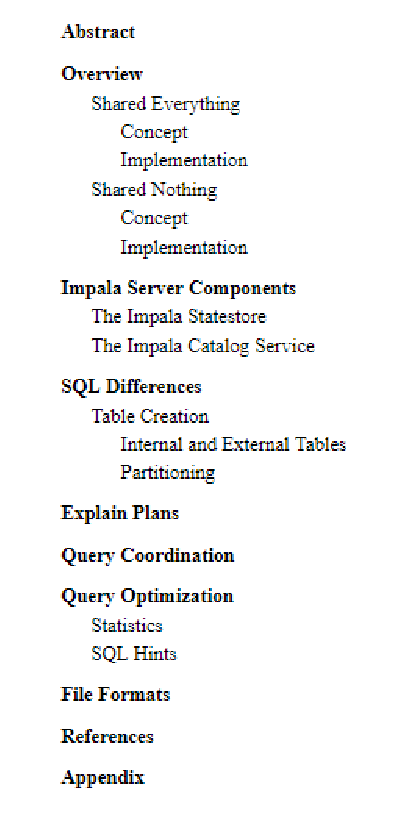
\includegraphics[width=\linewidth, height=4in, keepaspectratio]{ToC.eps}
\end{figure}

\subsection{Research Focus}
\subsubsection{Apache Impala Guide}
Throughout the term, we have been referring to Cloudera’s latest documentation for Apache Impala to research Impala’s inner workings.
The Apache Impala Guide is a comprehensive guide to every topic related to Impala, from installation and architecture to administration and optimization.
It is approximately 770 pages, which means it contains more detail than is necessary for engineers at HP to start working with the system.
It is also not specifically tailored towards engineers moving from an Oracle system to Impala, which is what HP’s engineers are doing.
While it is a good comprehensive guide filled with many fine details about the structure and operation of Impala, it is still missing some important information, such as details about the Statestore daemon, which our team had to look elsewhere to find information on. 
\subsubsection{Impala Server Components}
Impala is bundled with services that assist the Hadoop Distributed File System.
The services within the Impala ecosystem are intended to increase the overall performance of query execution through coordination between impala nodes.
Impala also possesses a number of optional services, which help to produce and optimize components of the service.
The two predominant services are the Statestore and the Impala Catalog Service. 

The Impala Statestore is a mandatory service for the Impala distributed system.
It must be running at all times, and if it is not, queries that involve nodes other than the initiator will not be able to resolve.
The Statestore acts as an arbitrator of the system, giving each node the information it needs to resolve a query, as well as keeping each individual node up to date with the most recent data commits.
Impala also uses the Statestore as a lexicon to interface with the other services that assist in improving impala’s performance, one of those services being the Impala Catalog Service. 

Impala’s Catalog Service is a daemon that is focused on the collection and update of metadata.
Metadata is collected from each node, and is placed into a central repository called the Metastore, which is shared within the service.
In application, the service acts as a listener for any DDL/DML changes within the Impala system.
When the Catalog Service detects a change, it grabs the new information and interfaces with the statestore to update the Metastore.
The service is a non-vital portion of the Impala ecosystem, and as such is an optional tool.
Its effects can be replicated by appending a REFRESH command after every SQL commit.

\subsubsection{SQL Differences}
The type of SQL used by Impala is known as HiveQL; while it conforms to the 2016 ANSI SQL standard, there are differences between the SQL currently used by the BackOffice team and HiveQL.
This section of the document is intended to point out areas where those changes may produce confusion or difficulty when transitioning.

A notable entry in this section are changes in the method of partitioning.
Oracle allows three methods of partitioning large tables: value, range, and hash partitioning.
However, Impala allows only value partitioning.
Methods for simulating the disallowed partition strategies are discussed, and syntax for implementing partitions is given. 

Also discussed in this section are the Impala definitions of internal and external tables.
Oracle also makes use of internal and external tables, but in a more limited fashion than Impala.
The methods for creating both kinds of tables are discussed, as well as the management of the files during updates, inserts, deletes, and drops. 

Planned additions to this section are a discussion of analytic functions, which are heavily used by HP when handling their data.
This section will seek to identify functions that are supported in Oracle’s SQL but not in HiveQL, as well as any differences in syntax or behavior across versions. 

\subsubsection{Query Optimization}
Through this term, we discovered that most query optimization hinges on the statistics of the data being queried.
The number of rows in a dataset is particularly important, as this directly shows how much data needs to be processed.
The amount of data to be processed, along with other  affects the type of JOIN operation Impala’s internal query optimizer uses in the query processing.
An incorrectly chosen JOIN operation can result in a query taking much longer than it should to be processed. 

Several commands exist to compute and modify data table statistics. The simplest of these commands is the COMPUTE STATS [Table\_Name] command. 

An engineer can manually change table statistics to influence the query optimizer’s choices.
An engineer can also include SQL hints within their queries to influence the query optimizer.
Such hints are also available in Oracle systems, and the differences between the two systems’ SQL hint coverage is discussed in this section.  

\subsubsection{File Formats}
In this term, we looked into several file formats that used in Apache Hadoop, which are Avro, Parquet and Optimized Row Columnar (ORC). Each of these file formats is unique and has their own relative advantages and disadvantages. It is important to choose file format used in Impala table since file format has significant impacts on the performance. For example, some file formats enable compression that may affect size of data and consequently lead to I/O and CPU resources required to deserialize data.
 
Parquet and ORC are column based file format, and Avro is row major file format. We found that Parquet is a good choice when you need to query a specific column with wide table, or work on some aggregation operations such as SUM() and AVG() that need to process most of the values in a column. Parquet table can also minimize I/O by reading less data and retrieve values from column quickly.
 
ORC is an optimized version of RCFile. However, Impala does not support it. It makes improvement on the compression by using an encoder that handle different column data types. ORC also skips blocks of rows that are not needed in query and then indexing fewer files and reduce load. This is why ORC has the better compression than Avro and Parquet.
 
Avro is a row major file format. Impala can query and create Avro tables, but not insert them. Avro schemas are defined with JSON and so it stores data definition in JSON after creating Avro tables. Currently, Avro tables do not support TIMESTAMP columns, but there are two functions that help to store time values. For some reason, mismatch of values type may occured between Avro schema and column definition in the database. To solve this problem, Impala uses schema reconciliation to check mismatching number of columns.


\subsection{Weekly Progress}
\begin{tabular}{l | p{15 cm}}
    Week & Details  \\ \hline
    Week 1 & During Week 1, we scheduled meeting times with our client, and had our first interactions with an Impala test environment. We discussed research topics for the term, and planned our initial topics. \\
    Week 2 & We discussed our initial research topics, and discussed the change in Impala interface. An HP employee has donated use of a server in their home to run a single-node Impala instance. This will allow us to use and investigate Impala without concern for cost. Our previous alternative was AWS, which requires paying for all server uptime. We discussed our elevator pitches, as well as our research for the week, including the catalogd daemon. \\
    Week 3 & Our client meeting this week was cancelled due to our client having car troubles, resulting in them being unable to make it. We rescheduled the meeting for Monday of next week. In the meantime, we investigated various related Hadoop components, and continued investigation of the catalogd daemon. \\
    Week 4 & We had two meetings this week to make up for the missed meeting in the previous week. We investigate partitioning, file formats, the statestored and catalogd. We set a goal of having an outline of the system comparison paper for our next meeting, to begin writing and review of our final document. \\
    Week 5 & Nate and Andy gave us some help with our difficulties inserting images into the .tex file of our document. We resolved the issue by converting the images to .eps files. We reviewed the outline and section headings of our final paper, as well as elevator pitch drafts and poster ideas. We have had some difficulty coordinating the poster review, but it was scheduled for the following week.  \\
    Week 6 & Nathaniel Whitlock reviewed parts of our rough draft for our final paper. During this work meeting we researched into SQL differences and query optimization to better fill out those sections in the paper. Nathaniel also clarified our questions in regard to the paper’s audience and purpose, and so we planned to tailor the paper more towards HP’s engineers, who have some background on SQL and relational databases, and are coming from a background of working with Oracle systems. We also took part in the initial poster critiques with team 67. Both teams gave insightful and helpful comments on each other’s posters and we came out of the meeting with more ideas for what needs to be on our poster.  \\
    Week 7 & We reviewed our rough (alpha) draft of our final paper with Andy Weiss and Nathaniel Whitlock. They made suggestions, corrections, and answered our questions as they read through the paper. In particular, Andy was able to find a more detailed price range for the new system that we could use to demonstrate its cost efficiency when presenting to the public. Going forward we will follow their suggestions to fix inconsistencies and expand on certain sections.  \\
\end{tabular}

\nocite{*}
\bibliographystyle{IEEEtran}
\bibliography{references}

\end{document}
